% Options for packages loaded elsewhere
\PassOptionsToPackage{unicode}{hyperref}
\PassOptionsToPackage{hyphens}{url}
%
\documentclass[
]{article}
\usepackage{amsmath,amssymb}
\usepackage{iftex}
\ifPDFTeX
  \usepackage[T1]{fontenc}
  \usepackage[utf8]{inputenc}
  \usepackage{textcomp} % provide euro and other symbols
\else % if luatex or xetex
  \usepackage{unicode-math} % this also loads fontspec
  \defaultfontfeatures{Scale=MatchLowercase}
  \defaultfontfeatures[\rmfamily]{Ligatures=TeX,Scale=1}
\fi
\usepackage{lmodern}
\ifPDFTeX\else
  % xetex/luatex font selection
\fi
% Use upquote if available, for straight quotes in verbatim environments
\IfFileExists{upquote.sty}{\usepackage{upquote}}{}
\IfFileExists{microtype.sty}{% use microtype if available
  \usepackage[]{microtype}
  \UseMicrotypeSet[protrusion]{basicmath} % disable protrusion for tt fonts
}{}
\makeatletter
\@ifundefined{KOMAClassName}{% if non-KOMA class
  \IfFileExists{parskip.sty}{%
    \usepackage{parskip}
  }{% else
    \setlength{\parindent}{0pt}
    \setlength{\parskip}{6pt plus 2pt minus 1pt}}
}{% if KOMA class
  \KOMAoptions{parskip=half}}
\makeatother
\usepackage{xcolor}
\usepackage[margin=1in]{geometry}
\usepackage{color}
\usepackage{fancyvrb}
\newcommand{\VerbBar}{|}
\newcommand{\VERB}{\Verb[commandchars=\\\{\}]}
\DefineVerbatimEnvironment{Highlighting}{Verbatim}{commandchars=\\\{\}}
% Add ',fontsize=\small' for more characters per line
\usepackage{framed}
\definecolor{shadecolor}{RGB}{248,248,248}
\newenvironment{Shaded}{\begin{snugshade}}{\end{snugshade}}
\newcommand{\AlertTok}[1]{\textcolor[rgb]{0.94,0.16,0.16}{#1}}
\newcommand{\AnnotationTok}[1]{\textcolor[rgb]{0.56,0.35,0.01}{\textbf{\textit{#1}}}}
\newcommand{\AttributeTok}[1]{\textcolor[rgb]{0.13,0.29,0.53}{#1}}
\newcommand{\BaseNTok}[1]{\textcolor[rgb]{0.00,0.00,0.81}{#1}}
\newcommand{\BuiltInTok}[1]{#1}
\newcommand{\CharTok}[1]{\textcolor[rgb]{0.31,0.60,0.02}{#1}}
\newcommand{\CommentTok}[1]{\textcolor[rgb]{0.56,0.35,0.01}{\textit{#1}}}
\newcommand{\CommentVarTok}[1]{\textcolor[rgb]{0.56,0.35,0.01}{\textbf{\textit{#1}}}}
\newcommand{\ConstantTok}[1]{\textcolor[rgb]{0.56,0.35,0.01}{#1}}
\newcommand{\ControlFlowTok}[1]{\textcolor[rgb]{0.13,0.29,0.53}{\textbf{#1}}}
\newcommand{\DataTypeTok}[1]{\textcolor[rgb]{0.13,0.29,0.53}{#1}}
\newcommand{\DecValTok}[1]{\textcolor[rgb]{0.00,0.00,0.81}{#1}}
\newcommand{\DocumentationTok}[1]{\textcolor[rgb]{0.56,0.35,0.01}{\textbf{\textit{#1}}}}
\newcommand{\ErrorTok}[1]{\textcolor[rgb]{0.64,0.00,0.00}{\textbf{#1}}}
\newcommand{\ExtensionTok}[1]{#1}
\newcommand{\FloatTok}[1]{\textcolor[rgb]{0.00,0.00,0.81}{#1}}
\newcommand{\FunctionTok}[1]{\textcolor[rgb]{0.13,0.29,0.53}{\textbf{#1}}}
\newcommand{\ImportTok}[1]{#1}
\newcommand{\InformationTok}[1]{\textcolor[rgb]{0.56,0.35,0.01}{\textbf{\textit{#1}}}}
\newcommand{\KeywordTok}[1]{\textcolor[rgb]{0.13,0.29,0.53}{\textbf{#1}}}
\newcommand{\NormalTok}[1]{#1}
\newcommand{\OperatorTok}[1]{\textcolor[rgb]{0.81,0.36,0.00}{\textbf{#1}}}
\newcommand{\OtherTok}[1]{\textcolor[rgb]{0.56,0.35,0.01}{#1}}
\newcommand{\PreprocessorTok}[1]{\textcolor[rgb]{0.56,0.35,0.01}{\textit{#1}}}
\newcommand{\RegionMarkerTok}[1]{#1}
\newcommand{\SpecialCharTok}[1]{\textcolor[rgb]{0.81,0.36,0.00}{\textbf{#1}}}
\newcommand{\SpecialStringTok}[1]{\textcolor[rgb]{0.31,0.60,0.02}{#1}}
\newcommand{\StringTok}[1]{\textcolor[rgb]{0.31,0.60,0.02}{#1}}
\newcommand{\VariableTok}[1]{\textcolor[rgb]{0.00,0.00,0.00}{#1}}
\newcommand{\VerbatimStringTok}[1]{\textcolor[rgb]{0.31,0.60,0.02}{#1}}
\newcommand{\WarningTok}[1]{\textcolor[rgb]{0.56,0.35,0.01}{\textbf{\textit{#1}}}}
\usepackage{graphicx}
\makeatletter
\def\maxwidth{\ifdim\Gin@nat@width>\linewidth\linewidth\else\Gin@nat@width\fi}
\def\maxheight{\ifdim\Gin@nat@height>\textheight\textheight\else\Gin@nat@height\fi}
\makeatother
% Scale images if necessary, so that they will not overflow the page
% margins by default, and it is still possible to overwrite the defaults
% using explicit options in \includegraphics[width, height, ...]{}
\setkeys{Gin}{width=\maxwidth,height=\maxheight,keepaspectratio}
% Set default figure placement to htbp
\makeatletter
\def\fps@figure{htbp}
\makeatother
\setlength{\emergencystretch}{3em} % prevent overfull lines
\providecommand{\tightlist}{%
  \setlength{\itemsep}{0pt}\setlength{\parskip}{0pt}}
\setcounter{secnumdepth}{-\maxdimen} % remove section numbering
\ifLuaTeX
  \usepackage{selnolig}  % disable illegal ligatures
\fi
\IfFileExists{bookmark.sty}{\usepackage{bookmark}}{\usepackage{hyperref}}
\IfFileExists{xurl.sty}{\usepackage{xurl}}{} % add URL line breaks if available
\urlstyle{same}
\hypersetup{
  pdftitle={Class Activity},
  pdfauthor={STAT380},
  hidelinks,
  pdfcreator={LaTeX via pandoc}}

\title{Class Activity}
\author{STAT380}
\date{}

\begin{document}
\maketitle

\begin{Shaded}
\begin{Highlighting}[]
\DocumentationTok{\#\#\#}
\FunctionTok{library}\NormalTok{(tree)}
\DocumentationTok{\#\#\#}
\FunctionTok{library}\NormalTok{(ISLR)}
\CommentTok{\#attach(Carseats)}
\FunctionTok{library}\NormalTok{(rattle)}
\end{Highlighting}
\end{Shaded}

\begin{verbatim}
## Warning: package 'rattle' was built under R version 4.0.5
\end{verbatim}

\begin{verbatim}
## Loading required package: tibble
\end{verbatim}

\begin{verbatim}
## Loading required package: bitops
\end{verbatim}

\begin{verbatim}
## Rattle: A free graphical interface for data science with R.
## Version 5.5.1 Copyright (c) 2006-2021 Togaware Pty Ltd.
## Type 'rattle()' to shake, rattle, and roll your data.
\end{verbatim}

\begin{Shaded}
\begin{Highlighting}[]
\FunctionTok{library}\NormalTok{(rpart.plot)}
\end{Highlighting}
\end{Shaded}

\begin{verbatim}
## Loading required package: rpart
\end{verbatim}

\begin{Shaded}
\begin{Highlighting}[]
\FunctionTok{library}\NormalTok{(RColorBrewer)}
\FunctionTok{library}\NormalTok{(partykit)}
\end{Highlighting}
\end{Shaded}

\begin{verbatim}
## Loading required package: grid
\end{verbatim}

\begin{verbatim}
## Loading required package: libcoin
\end{verbatim}

\begin{verbatim}
## Loading required package: mvtnorm
\end{verbatim}

\#(Fitting Regression Trees)

\hypertarget{we-will-use-the-classification-trees-for-the-boston-housing-data}{%
\subsubsection{We will use the classification trees for the Boston
Housing
data}\label{we-will-use-the-classification-trees-for-the-boston-housing-data}}

Load the data from the github course page using:

\begin{Shaded}
\begin{Highlighting}[]
\NormalTok{BostonHousing}\OtherTok{\textless{}{-}}\FunctionTok{read.csv}\NormalTok{(}\FunctionTok{url}\NormalTok{(}\StringTok{"https://raw.githubusercontent.com/subhadippal2019/STAT380UAEU/main/BostonHousing.csv"}\NormalTok{))}
\FunctionTok{names}\NormalTok{(BostonHousing)}
\end{Highlighting}
\end{Shaded}

\begin{verbatim}
##  [1] "CRIM"      "ZN"        "INDUS"     "CHAS"      "NOX"       "RM"       
##  [7] "AGE"       "DIS"       "RAD"       "TAX"       "PTRATIO"   "LSTAT"    
## [13] "MEDV"      "CAT..MEDV"
\end{verbatim}

\#\#Some notations Some notations on the response variable and
additional information on Data. Also remove the continuous response,
\texttt{MEDV\textquotesingle{}\ as\ objective\ of\ this\ activity\ is\ to\ construct\ a\ Classification\ tree\ on\ the\ categorical\ covariate}CAT..MEDV'

\begin{Shaded}
\begin{Highlighting}[]
\DocumentationTok{\#\# Classification tree using Boston Housing data: }
\CommentTok{\# Some notation and additional information on Data}
\FunctionTok{head}\NormalTok{(BostonHousing)}
\end{Highlighting}
\end{Shaded}

\begin{verbatim}
##      CRIM ZN INDUS CHAS   NOX    RM  AGE    DIS RAD TAX PTRATIO LSTAT MEDV
## 1 0.00632 18  2.31    0 0.538 6.575 65.2 4.0900   1 296    15.3  4.98 24.0
## 2 0.02731  0  7.07    0 0.469 6.421 78.9 4.9671   2 242    17.8  9.14 21.6
## 3 0.02729  0  7.07    0 0.469 7.185 61.1 4.9671   2 242    17.8  4.03 34.7
## 4 0.03237  0  2.18    0 0.458 6.998 45.8 6.0622   3 222    18.7  2.94 33.4
## 5 0.06905  0  2.18    0 0.458 7.147 54.2 6.0622   3 222    18.7  5.33 36.2
## 6 0.02985  0  2.18    0 0.458 6.430 58.7 6.0622   3 222    18.7  5.21 28.7
##   CAT..MEDV
## 1         0
## 2         0
## 3         1
## 4         1
## 5         1
## 6         0
\end{verbatim}

\begin{Shaded}
\begin{Highlighting}[]
\FunctionTok{str}\NormalTok{(BostonHousing)}
\end{Highlighting}
\end{Shaded}

\begin{verbatim}
## 'data.frame':    506 obs. of  14 variables:
##  $ CRIM     : num  0.00632 0.02731 0.02729 0.03237 0.06905 ...
##  $ ZN       : num  18 0 0 0 0 0 12.5 12.5 12.5 12.5 ...
##  $ INDUS    : num  2.31 7.07 7.07 2.18 2.18 2.18 7.87 7.87 7.87 7.87 ...
##  $ CHAS     : int  0 0 0 0 0 0 0 0 0 0 ...
##  $ NOX      : num  0.538 0.469 0.469 0.458 0.458 0.458 0.524 0.524 0.524 0.524 ...
##  $ RM       : num  6.58 6.42 7.18 7 7.15 ...
##  $ AGE      : num  65.2 78.9 61.1 45.8 54.2 58.7 66.6 96.1 100 85.9 ...
##  $ DIS      : num  4.09 4.97 4.97 6.06 6.06 ...
##  $ RAD      : int  1 2 2 3 3 3 5 5 5 5 ...
##  $ TAX      : int  296 242 242 222 222 222 311 311 311 311 ...
##  $ PTRATIO  : num  15.3 17.8 17.8 18.7 18.7 18.7 15.2 15.2 15.2 15.2 ...
##  $ LSTAT    : num  4.98 9.14 4.03 2.94 5.33 ...
##  $ MEDV     : num  24 21.6 34.7 33.4 36.2 28.7 22.9 27.1 16.5 18.9 ...
##  $ CAT..MEDV: int  0 0 1 1 1 0 0 0 0 0 ...
\end{verbatim}

\begin{Shaded}
\begin{Highlighting}[]
\NormalTok{BostonHousing}\SpecialCharTok{$}\NormalTok{MEDV\_Fac }\OtherTok{=} \FunctionTok{factor}\NormalTok{(BostonHousing}\SpecialCharTok{$}\NormalTok{CAT..MEDV,}\AttributeTok{labels=}\FunctionTok{c}\NormalTok{(}\StringTok{"Below"}\NormalTok{,}\StringTok{"Above"}\NormalTok{))}
\NormalTok{BostonHousing}\SpecialCharTok{$}\NormalTok{MEDV\_Fac}
\end{Highlighting}
\end{Shaded}

\begin{verbatim}
##   [1] Below Below Above Above Above Below Below Below Below Below Below Below
##  [13] Below Below Below Below Below Below Below Below Below Below Below Below
##  [25] Below Below Below Below Below Below Below Below Below Below Below Below
##  [37] Below Below Below Above Above Below Below Below Below Below Below Below
##  [49] Below Below Below Below Below Below Below Above Below Above Below Below
##  [61] Below Below Below Below Above Below Below Below Below Below Below Below
##  [73] Below Below Below Below Below Below Below Below Below Below Below Below
##  [85] Below Below Below Below Below Below Below Below Below Below Below Below
##  [97] Below Above Above Above Below Below Below Below Below Below Below Below
## [109] Below Below Below Below Below Below Below Below Below Below Below Below
## [121] Below Below Below Below Below Below Below Below Below Below Below Below
## [133] Below Below Below Below Below Below Below Below Below Below Below Below
## [145] Below Below Below Below Below Below Below Below Below Below Below Below
## [157] Below Above Below Below Below Above Above Above Below Below Above Below
## [169] Below Below Below Below Below Below Below Below Below Below Below Above
## [181] Above Above Above Above Below Below Above Above Below Above Above Above
## [193] Above Above Below Above Above Above Above Above Above Below Above Above
## [205] Above Below Below Below Below Below Below Below Below Below Below Below
## [217] Below Below Below Below Below Below Below Above Above Above Above Above
## [229] Above Above Below Above Above Above Below Below Below Above Below Below
## [241] Below Below Below Below Below Below Below Below Below Below Below Below
## [253] Below Above Below Below Above Above Above Above Above Above Above Above
## [265] Above Below Above Above Above Below Below Below Below Above Above Above
## [277] Above Above Below Above Above Above Above Above Above Below Below Below
## [289] Below Below Below Above Below Below Below Below Below Below Below Below
## [301] Below Below Below Above Above Below Above Below Below Below Below Below
## [313] Below Below Below Below Below Below Below Below Below Below Below Below
## [325] Below Below Below Below Below Below Below Below Below Below Below Below
## [337] Below Below Below Below Below Above Below Below Above Below Below Below
## [349] Below Below Below Below Below Above Below Below Below Below Below Below
## [361] Below Below Below Below Below Below Below Below Above Above Above Above
## [373] Above Below Below Below Below Below Below Below Below Below Below Below
## [385] Below Below Below Below Below Below Below Below Below Below Below Below
## [397] Below Below Below Below Below Below Below Below Below Below Below Below
## [409] Below Below Below Below Below Below Below Below Below Below Below Below
## [421] Below Below Below Below Below Below Below Below Below Below Below Below
## [433] Below Below Below Below Below Below Below Below Below Below Below Below
## [445] Below Below Below Below Below Below Below Below Below Below Below Below
## [457] Below Below Below Below Below Below Below Below Below Below Below Below
## [469] Below Below Below Below Below Below Below Below Below Below Below Below
## [481] Below Below Below Below Below Below Below Below Below Below Below Below
## [493] Below Below Below Below Below Below Below Below Below Below Below Below
## [505] Below Below
## Levels: Below Above
\end{verbatim}

\begin{Shaded}
\begin{Highlighting}[]
\CommentTok{\# As we will be using the MEDV\_Fac as categorical response, we will remove both, \textasciigrave{}CAT..MEDV\textquotesingle{} and \textasciigrave{}MEDV\textquotesingle{} to keep on the required of the data. }
\NormalTok{BostonH}\OtherTok{=}\NormalTok{BostonHousing[,}\SpecialCharTok{{-}}\FunctionTok{c}\NormalTok{(}\DecValTok{13}\NormalTok{,}\DecValTok{14}\NormalTok{)] }
\CommentTok{\#We will work on the BostonH for rest of the activity}
\end{Highlighting}
\end{Shaded}

\hypertarget{split-the-data-in-training-and-testing-set.-use-a-7030-split-for-the-training-and-testing-set.-print-the-dimension-of-the-testing-and-the-training-set.}{%
\subsubsection{Split the data in Training and Testing Set. Use a
70\%/30\% split for the Training and Testing Set. Print the dimension of
the Testing and the Training
set.}\label{split-the-data-in-training-and-testing-set.-use-a-7030-split-for-the-training-and-testing-set.-print-the-dimension-of-the-testing-and-the-training-set.}}

\begin{Shaded}
\begin{Highlighting}[]
\DocumentationTok{\#\#\#\# A5.1:}
\FunctionTok{set.seed}\NormalTok{(}\DecValTok{234}\NormalTok{)}
 \CommentTok{\#inTrain = createDataPartition(Carseats$Sales, p = 0.6, list = FALSE)}
\NormalTok{  Total\_data\_size}\OtherTok{=}\FunctionTok{as.integer}\NormalTok{(}\FunctionTok{nrow}\NormalTok{(BostonH))}
\NormalTok{  inTrain }\OtherTok{=} \FunctionTok{sample}\NormalTok{(}\DecValTok{1}\SpecialCharTok{:}\NormalTok{Total\_data\_size, }\FunctionTok{round}\NormalTok{(Total\_data\_size}\SpecialCharTok{*}\FloatTok{0.70}\NormalTok{))}
\NormalTok{  Training\_Set }\OtherTok{=}\NormalTok{ BostonH[inTrain, ]}
  \FunctionTok{dim}\NormalTok{(Training\_Set)}
\end{Highlighting}
\end{Shaded}

\begin{verbatim}
## [1] 354  13
\end{verbatim}

\begin{Shaded}
\begin{Highlighting}[]
\NormalTok{  Testing\_Set}\OtherTok{\textless{}{-}}\NormalTok{BostonH[}\SpecialCharTok{{-}}\NormalTok{inTrain, ]}
  \FunctionTok{dim}\NormalTok{(Testing\_Set)}
\end{Highlighting}
\end{Shaded}

\begin{verbatim}
## [1] 152  13
\end{verbatim}

\begin{Shaded}
\begin{Highlighting}[]
  \FunctionTok{names}\NormalTok{(BostonH)}
\end{Highlighting}
\end{Shaded}

\begin{verbatim}
##  [1] "CRIM"     "ZN"       "INDUS"    "CHAS"     "NOX"      "RM"      
##  [7] "AGE"      "DIS"      "RAD"      "TAX"      "PTRATIO"  "LSTAT"   
## [13] "MEDV_Fac"
\end{verbatim}

\hypertarget{fitting-a-classification-tree}{%
\subsubsection{Fitting a classification
Tree}\label{fitting-a-classification-tree}}

We Fit a classification tree on the Training Set using the response
`MEDV\_Fac', the median price of houses in a region, as the response
variable while all the other variables. We also Display/plot the fitted
tree.

\begin{Shaded}
\begin{Highlighting}[]
\CommentTok{\#{-}{-}{-}{-}{-}{-}{-}{-}{-}{-}{-}{-}{-}{-}{-}{-}{-}{-}{-}{-}{-}{-}{-}{-}{-}{-}{-}{-}{-}{-}{-}{-}{-}{-}{-}{-}{-}}
\CommentTok{\# Grow a general classification tree with multiple covariates}
\CommentTok{\# {-} minimum number of units that exists in a node in order for a split to be attempted}
\CommentTok{\# {-} change complexity parameter alpha to {-}1 {-} full tree}
\FunctionTok{set.seed}\NormalTok{(}\DecValTok{12043}\NormalTok{)}
\NormalTok{cls\_fit\_train }\OtherTok{=} \FunctionTok{rpart}\NormalTok{(MEDV\_Fac}\SpecialCharTok{\textasciitilde{}}\NormalTok{CRIM}\SpecialCharTok{+}\NormalTok{ZN}\SpecialCharTok{+}\NormalTok{INDUS}\SpecialCharTok{+}\NormalTok{CHAS}\SpecialCharTok{+}\NormalTok{NOX}\SpecialCharTok{+}\NormalTok{RM}\SpecialCharTok{+}\NormalTok{AGE}\SpecialCharTok{+}\NormalTok{DIS}\SpecialCharTok{+}\NormalTok{RAD}\SpecialCharTok{+}\NormalTok{TAX}\SpecialCharTok{+}\NormalTok{PTRATIO}\SpecialCharTok{+}\NormalTok{LSTAT,}\AttributeTok{data=}\NormalTok{Training\_Set,}\AttributeTok{method=}\StringTok{"class"}\NormalTok{,}\AttributeTok{minsplit=}\DecValTok{5}\NormalTok{,}\AttributeTok{cp=}\DecValTok{0}\NormalTok{)}

\CommentTok{\# plot fitted tree\# You may use fancyRpartPlot(fitted\_object, caption = NULL)}
\FunctionTok{fancyRpartPlot}\NormalTok{(cls\_fit\_train, }\AttributeTok{caption =} \ConstantTok{NULL}\NormalTok{)}
\end{Highlighting}
\end{Shaded}

\includegraphics{R_codes_Trees_-imp-for-Assignemnt2-1_files/figure-latex/unnamed-chunk-5-1.pdf}

\hypertarget{print-the-summary-and-the-tables-containig-the-crossvalidated-cp-and-plot-the-crossvalidatedcp.-summary-printcp-plotcp-we-also-identify-an-optimal-value-for-the-complexity-parameter-cp.}{%
\subsubsection{\texorpdfstring{Print the summary and the tables
containig the crossvalidated
`\texttt{cp\textquotesingle{}\ and\ plot\ the\ \textasciigrave{}crossvalidated}cp'.
(summary, printcp, plotcp) We also, identify an optimal value for the
complexity parameter
`cp'.}{Print the summary and the tables containig the crossvalidated `cp\textquotesingle{} and plot the `crossvalidatedcp'. (summary, printcp, plotcp) We also, identify an optimal value for the complexity parameter `cp'.}}\label{print-the-summary-and-the-tables-containig-the-crossvalidated-cp-and-plot-the-crossvalidatedcp.-summary-printcp-plotcp-we-also-identify-an-optimal-value-for-the-complexity-parameter-cp.}}

\begin{Shaded}
\begin{Highlighting}[]
\FunctionTok{summary}\NormalTok{(cls\_fit\_train)}
\end{Highlighting}
\end{Shaded}

\begin{verbatim}
## Call:
## rpart(formula = MEDV_Fac ~ CRIM + ZN + INDUS + CHAS + NOX + RM + 
##     AGE + DIS + RAD + TAX + PTRATIO + LSTAT, data = Training_Set, 
##     method = "class", minsplit = 5, cp = 0)
##   n= 354 
## 
##           CP nsplit  rel error    xerror       xstd
## 1 0.62295082      0 1.00000000 1.0000000 0.11648426
## 2 0.18032787      1 0.37704918 0.5409836 0.08967637
## 3 0.03278689      2 0.19672131 0.3442623 0.07286187
## 4 0.01639344      3 0.16393443 0.2786885 0.06594896
## 5 0.01092896      7 0.08196721 0.3278689 0.07121259
## 6 0.00000000     10 0.04918033 0.3278689 0.07121259
## 
## Variable importance
##      RM   LSTAT PTRATIO      ZN   INDUS    CRIM     NOX     TAX     RAD     DIS 
##      35      25       8       6       5       5       5       4       4       2 
##     AGE 
##       1 
## 
## Node number 1: 354 observations,    complexity param=0.6229508
##   predicted class=Below  expected loss=0.1723164  P(node) =1
##     class counts:   293    61
##    probabilities: 0.828 0.172 
##   left son=2 (312 obs) right son=3 (42 obs)
##   Primary splits:
##       RM      < 7.0835   to the left,  improve=57.99480, (0 missing)
##       LSTAT   < 5.055    to the right, improve=53.34461, (0 missing)
##       INDUS   < 3.985    to the right, improve=27.06907, (0 missing)
##       PTRATIO < 17.85    to the right, improve=17.20158, (0 missing)
##       ZN      < 15       to the left,  improve=12.82695, (0 missing)
##   Surrogate splits:
##       LSTAT   < 4.475    to the right, agree=0.921, adj=0.333, (0 split)
##       PTRATIO < 14.55    to the right, agree=0.898, adj=0.143, (0 split)
##       ZN      < 87.5     to the left,  agree=0.890, adj=0.071, (0 split)
##       INDUS   < 1.605    to the right, agree=0.887, adj=0.048, (0 split)
## 
## Node number 2: 312 observations,    complexity param=0.1803279
##   predicted class=Below  expected loss=0.06730769  P(node) =0.8813559
##     class counts:   291    21
##    probabilities: 0.933 0.067 
##   left son=4 (295 obs) right son=5 (17 obs)
##   Primary splits:
##       LSTAT < 4.695    to the right, improve=20.564100, (0 missing)
##       RM    < 6.6805   to the left,  improve= 9.933946, (0 missing)
##       INDUS < 3.985    to the right, improve= 6.093665, (0 missing)
##       ZN    < 87.5     to the left,  improve= 5.270164, (0 missing)
##       CRIM  < 0.032715 to the right, improve= 3.668856, (0 missing)
##   Surrogate splits:
##       ZN    < 87.5     to the left,  agree=0.955, adj=0.176, (0 split)
##       INDUS < 1.58     to the right, agree=0.949, adj=0.059, (0 split)
## 
## Node number 3: 42 observations,    complexity param=0.03278689
##   predicted class=Above  expected loss=0.04761905  P(node) =0.1186441
##     class counts:     2    40
##    probabilities: 0.048 0.952 
##   left son=6 (2 obs) right son=7 (40 obs)
##   Primary splits:
##       CRIM    < 5.12914  to the right, improve=3.809524, (0 missing)
##       NOX     < 0.659    to the right, improve=3.809524, (0 missing)
##       RAD     < 16       to the right, improve=3.809524, (0 missing)
##       TAX     < 534.5    to the right, improve=3.809524, (0 missing)
##       PTRATIO < 19.4     to the right, improve=3.809524, (0 missing)
##   Surrogate splits:
##       NOX     < 0.659    to the right, agree=1, adj=1, (0 split)
##       RAD     < 16       to the right, agree=1, adj=1, (0 split)
##       TAX     < 534.5    to the right, agree=1, adj=1, (0 split)
##       PTRATIO < 19.4     to the right, agree=1, adj=1, (0 split)
##       LSTAT   < 12.345   to the right, agree=1, adj=1, (0 split)
## 
## Node number 4: 295 observations,    complexity param=0.01639344
##   predicted class=Below  expected loss=0.02372881  P(node) =0.8333333
##     class counts:   288     7
##    probabilities: 0.976 0.024 
##   left son=8 (253 obs) right son=9 (42 obs)
##   Primary splits:
##       RM      < 6.5545   to the left,  improve=1.3899870, (0 missing)
##       INDUS   < 3.985    to the right, improve=1.3110030, (0 missing)
##       LSTAT   < 5.055    to the right, improve=1.1741400, (0 missing)
##       DIS     < 1.1556   to the right, improve=0.9135304, (0 missing)
##       PTRATIO < 13.85    to the right, improve=0.9135304, (0 missing)
##   Surrogate splits:
##       LSTAT < 5.055    to the right, agree=0.878, adj=0.143, (0 split)
##       NOX   < 0.403    to the right, agree=0.861, adj=0.024, (0 split)
## 
## Node number 5: 17 observations,    complexity param=0.01092896
##   predicted class=Above  expected loss=0.1764706  P(node) =0.0480226
##     class counts:     3    14
##    probabilities: 0.176 0.824 
##   left son=10 (8 obs) right son=11 (9 obs)
##   Primary splits:
##       RAD     < 4.5      to the left,  improve=1.1911760, (0 missing)
##       ZN      < 77.5     to the right, improve=0.7078431, (0 missing)
##       NOX     < 0.4195   to the left,  improve=0.7078431, (0 missing)
##       RM      < 6.659    to the left,  improve=0.7078431, (0 missing)
##       PTRATIO < 18.35    to the right, improve=0.7078431, (0 missing)
##   Surrogate splits:
##       AGE     < 28       to the left,  agree=0.765, adj=0.500, (0 split)
##       NOX     < 0.471    to the left,  agree=0.706, adj=0.375, (0 split)
##       TAX     < 255      to the left,  agree=0.706, adj=0.375, (0 split)
##       PTRATIO < 15.65    to the right, agree=0.706, adj=0.375, (0 split)
##       CRIM    < 0.036445 to the left,  agree=0.647, adj=0.250, (0 split)
## 
## Node number 6: 2 observations
##   predicted class=Below  expected loss=0  P(node) =0.005649718
##     class counts:     2     0
##    probabilities: 1.000 0.000 
## 
## Node number 7: 40 observations
##   predicted class=Above  expected loss=0  P(node) =0.1129944
##     class counts:     0    40
##    probabilities: 0.000 1.000 
## 
## Node number 8: 253 observations
##   predicted class=Below  expected loss=0.003952569  P(node) =0.7146893
##     class counts:   252     1
##    probabilities: 0.996 0.004 
## 
## Node number 9: 42 observations,    complexity param=0.01639344
##   predicted class=Below  expected loss=0.1428571  P(node) =0.1186441
##     class counts:    36     6
##    probabilities: 0.857 0.143 
##   left son=18 (40 obs) right son=19 (2 obs)
##   Primary splits:
##       TAX     < 219      to the right, improve=3.0857140, (0 missing)
##       PTRATIO < 15.8     to the right, improve=3.0857140, (0 missing)
##       INDUS   < 4.01     to the right, improve=1.9285710, (0 missing)
##       LSTAT   < 7.825    to the right, improve=1.5584420, (0 missing)
##       RAD     < 5.5      to the right, improve=0.8766234, (0 missing)
## 
## Node number 10: 8 observations,    complexity param=0.01092896
##   predicted class=Above  expected loss=0.375  P(node) =0.02259887
##     class counts:     3     5
##    probabilities: 0.375 0.625 
##   left son=20 (5 obs) right son=21 (3 obs)
##   Primary splits:
##       CRIM  < 0.033695 to the right, improve=1.3500000, (0 missing)
##       INDUS < 3.16     to the right, improve=1.3500000, (0 missing)
##       RAD   < 3.5      to the right, improve=1.3500000, (0 missing)
##       ZN    < 77.5     to the right, improve=0.8166667, (0 missing)
##       NOX   < 0.4195   to the left,  improve=0.8166667, (0 missing)
##   Surrogate splits:
##       INDUS < 3.16     to the right, agree=1.000, adj=1.000, (0 split)
##       RAD   < 3.5      to the right, agree=1.000, adj=1.000, (0 split)
##       RM    < 6.918    to the left,  agree=0.875, adj=0.667, (0 split)
##       DIS   < 5.2589   to the left,  agree=0.875, adj=0.667, (0 split)
##       AGE   < 24.7     to the right, agree=0.750, adj=0.333, (0 split)
## 
## Node number 11: 9 observations
##   predicted class=Above  expected loss=0  P(node) =0.02542373
##     class counts:     0     9
##    probabilities: 0.000 1.000 
## 
## Node number 18: 40 observations,    complexity param=0.01639344
##   predicted class=Below  expected loss=0.1  P(node) =0.1129944
##     class counts:    36     4
##    probabilities: 0.900 0.100 
##   left son=36 (34 obs) right son=37 (6 obs)
##   Primary splits:
##       PTRATIO < 15.8     to the right, improve=2.2588240, (0 missing)
##       LSTAT   < 7.825    to the right, improve=0.8000000, (0 missing)
##       INDUS   < 4.01     to the right, improve=0.7714286, (0 missing)
##       AGE     < 9.95     to the right, improve=0.6736842, (0 missing)
##       ZN      < 19       to the left,  improve=0.6586895, (0 missing)
##   Surrogate splits:
##       NOX  < 0.403    to the right, agree=0.925, adj=0.500, (0 split)
##       CRIM < 0.02862  to the right, agree=0.875, adj=0.167, (0 split)
##       ZN   < 39.5     to the left,  agree=0.875, adj=0.167, (0 split)
##       AGE  < 16.45    to the right, agree=0.875, adj=0.167, (0 split)
##       DIS  < 7.5725   to the left,  agree=0.875, adj=0.167, (0 split)
## 
## Node number 19: 2 observations
##   predicted class=Above  expected loss=0  P(node) =0.005649718
##     class counts:     0     2
##    probabilities: 0.000 1.000 
## 
## Node number 20: 5 observations,    complexity param=0.01092896
##   predicted class=Below  expected loss=0.4  P(node) =0.01412429
##     class counts:     3     2
##    probabilities: 0.600 0.400 
##   left son=40 (2 obs) right son=41 (3 obs)
##   Primary splits:
##       CRIM  < 0.048555 to the left,  improve=1.066667, (0 missing)
##       ZN    < 60       to the right, improve=1.066667, (0 missing)
##       INDUS < 5.68     to the left,  improve=1.066667, (0 missing)
##       NOX   < 0.429    to the left,  improve=1.066667, (0 missing)
##       RM    < 6.7305   to the left,  improve=1.066667, (0 missing)
##   Surrogate splits:
##       ZN    < 60       to the right, agree=1.0, adj=1.0, (0 split)
##       INDUS < 5.68     to the left,  agree=1.0, adj=1.0, (0 split)
##       NOX   < 0.429    to the left,  agree=1.0, adj=1.0, (0 split)
##       DIS   < 4.98975  to the right, agree=1.0, adj=1.0, (0 split)
##       AGE   < 35.35    to the left,  agree=0.8, adj=0.5, (0 split)
## 
## Node number 21: 3 observations
##   predicted class=Above  expected loss=0  P(node) =0.008474576
##     class counts:     0     3
##    probabilities: 0.000 1.000 
## 
## Node number 36: 34 observations
##   predicted class=Below  expected loss=0.02941176  P(node) =0.0960452
##     class counts:    33     1
##    probabilities: 0.971 0.029 
## 
## Node number 37: 6 observations,    complexity param=0.01639344
##   predicted class=Below  expected loss=0.5  P(node) =0.01694915
##     class counts:     3     3
##    probabilities: 0.500 0.500 
##   left son=74 (3 obs) right son=75 (3 obs)
##   Primary splits:
##       INDUS < 2.62     to the left,  improve=3.0, (0 missing)
##       CRIM  < 0.06718  to the left,  improve=1.5, (0 missing)
##       ZN    < 65       to the right, improve=1.5, (0 missing)
##       NOX   < 0.4005   to the left,  improve=1.5, (0 missing)
##       RM    < 6.8565   to the right, improve=1.5, (0 missing)
##   Surrogate splits:
##       CRIM < 0.06718  to the left,  agree=0.833, adj=0.667, (0 split)
##       ZN   < 65       to the right, agree=0.833, adj=0.667, (0 split)
##       NOX  < 0.4005   to the left,  agree=0.833, adj=0.667, (0 split)
##       RM   < 6.8565   to the right, agree=0.833, adj=0.667, (0 split)
##       DIS  < 3.9393   to the right, agree=0.833, adj=0.667, (0 split)
## 
## Node number 40: 2 observations
##   predicted class=Below  expected loss=0  P(node) =0.005649718
##     class counts:     2     0
##    probabilities: 1.000 0.000 
## 
## Node number 41: 3 observations
##   predicted class=Above  expected loss=0.3333333  P(node) =0.008474576
##     class counts:     1     2
##    probabilities: 0.333 0.667 
## 
## Node number 74: 3 observations
##   predicted class=Below  expected loss=0  P(node) =0.008474576
##     class counts:     3     0
##    probabilities: 1.000 0.000 
## 
## Node number 75: 3 observations
##   predicted class=Above  expected loss=0  P(node) =0.008474576
##     class counts:     0     3
##    probabilities: 0.000 1.000
\end{verbatim}

\begin{Shaded}
\begin{Highlighting}[]
\FunctionTok{printcp}\NormalTok{(cls\_fit\_train)}
\end{Highlighting}
\end{Shaded}

\begin{verbatim}
## 
## Classification tree:
## rpart(formula = MEDV_Fac ~ CRIM + ZN + INDUS + CHAS + NOX + RM + 
##     AGE + DIS + RAD + TAX + PTRATIO + LSTAT, data = Training_Set, 
##     method = "class", minsplit = 5, cp = 0)
## 
## Variables actually used in tree construction:
## [1] CRIM    INDUS   LSTAT   PTRATIO RAD     RM      TAX    
## 
## Root node error: 61/354 = 0.17232
## 
## n= 354 
## 
##         CP nsplit rel error  xerror     xstd
## 1 0.622951      0  1.000000 1.00000 0.116484
## 2 0.180328      1  0.377049 0.54098 0.089676
## 3 0.032787      2  0.196721 0.34426 0.072862
## 4 0.016393      3  0.163934 0.27869 0.065949
## 5 0.010929      7  0.081967 0.32787 0.071213
## 6 0.000000     10  0.049180 0.32787 0.071213
\end{verbatim}

\begin{Shaded}
\begin{Highlighting}[]
\FunctionTok{plotcp}\NormalTok{(cls\_fit\_train) }
\end{Highlighting}
\end{Shaded}

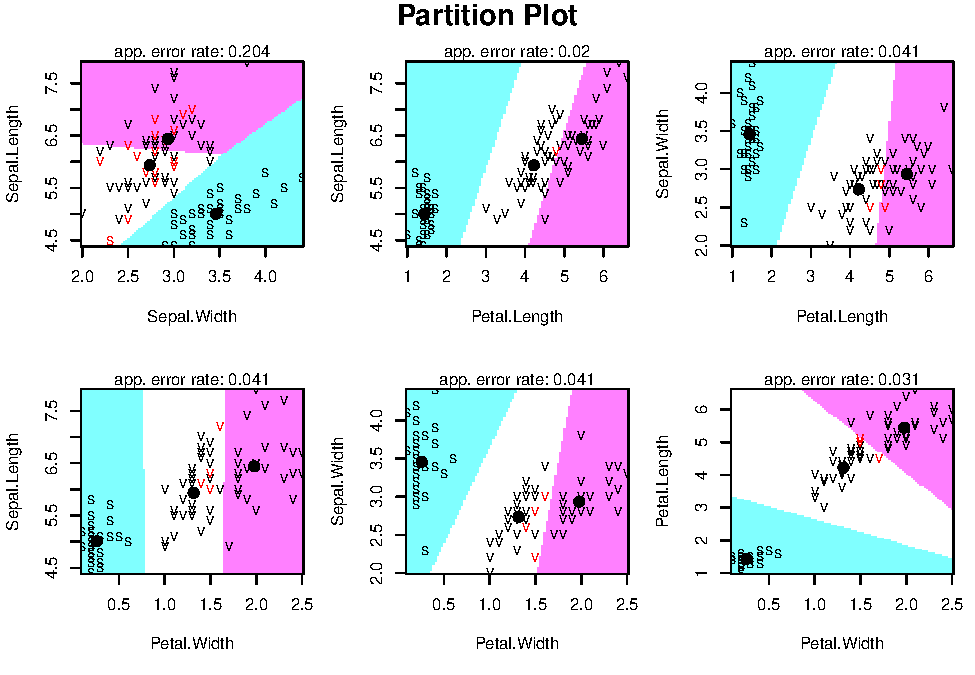
\includegraphics{R_codes_Trees_-imp-for-Assignemnt2-1_files/figure-latex/unnamed-chunk-6-1.pdf}

\hypertarget{section}{%
\subsubsection{}\label{section}}

\hypertarget{find-the-optimal-value-of-cp-and-prune-the-regression-tree.}{%
\subsection{Find the optimal value of `cp' and Prune the regression
tree.}\label{find-the-optimal-value-of-cp-and-prune-the-regression-tree.}}

\begin{Shaded}
\begin{Highlighting}[]
\DocumentationTok{\#\# B4.}
\NormalTok{bestcp }\OtherTok{\textless{}{-}}\NormalTok{cls\_fit\_train}\SpecialCharTok{$}\NormalTok{cptable[}\FunctionTok{which.min}\NormalTok{(cls\_fit\_train}\SpecialCharTok{$}\NormalTok{cptable[,}\StringTok{"xerror"}\NormalTok{]),}\StringTok{"CP"}\NormalTok{]}
\end{Highlighting}
\end{Shaded}

\hypertarget{section-1}{%
\subsubsection{}\label{section-1}}

\hypertarget{prune-the-regression-tree-to-find-the-optimal-number-of-nodes.}{%
\subsection{Prune the regression tree to find the optimal number of
nodes.}\label{prune-the-regression-tree-to-find-the-optimal-number-of-nodes.}}

\begin{Shaded}
\begin{Highlighting}[]
\CommentTok{\#bestcp \textless{}{-}fit\_train$cptable[which.min(fit\_train$cptable[,"xerror"]),"CP"]}
\NormalTok{cls\_pruned.tree }\OtherTok{\textless{}{-}} \FunctionTok{prune}\NormalTok{(cls\_fit\_train, }\AttributeTok{cp =}\NormalTok{ bestcp)}
\FunctionTok{rpart.plot}\NormalTok{(cls\_pruned.tree)}
\end{Highlighting}
\end{Shaded}

\includegraphics{R_codes_Trees_-imp-for-Assignemnt2-1_files/figure-latex/unnamed-chunk-8-1.pdf}
\#\#\#

\hypertarget{predict-on-the-testing-set-with-the-pruned-tree.-plot-the-predicted-values-vs-the-response-values-in-the-test-set.}{%
\subsection{Predict on the Testing set with the pruned tree. Plot the
predicted values vs the response values in the test
set.}\label{predict-on-the-testing-set-with-the-pruned-tree.-plot-the-predicted-values-vs-the-response-values-in-the-test-set.}}

\hypertarget{predict-on-the-testing-set-with-the-entire-tree-fitted-to-the-training-set.-plot-the-predicted-values-vs-the-response-values-in-the-test-set.}{%
\subsection{Predict on the Testing set with the Entire tree fitted to
the training set. Plot the predicted values vs the response values in
the test
set.}\label{predict-on-the-testing-set-with-the-entire-tree-fitted-to-the-training-set.-plot-the-predicted-values-vs-the-response-values-in-the-test-set.}}

\begin{Shaded}
\begin{Highlighting}[]
\DocumentationTok{\#\#Predict: }
\NormalTok{cls\_pred\_test.prune\_prob }\OtherTok{=} \FunctionTok{predict}\NormalTok{(cls\_pruned.tree, Testing\_Set)}

\NormalTok{cls\_pred\_test.prune }\OtherTok{=} \FunctionTok{predict}\NormalTok{(cls\_pruned.tree, Testing\_Set, }\AttributeTok{type=}\StringTok{"class"}\NormalTok{)}

\DocumentationTok{\#\#\# }
\NormalTok{cls\_pred\_test.full\_tree}\OtherTok{=}\FunctionTok{predict}\NormalTok{(cls\_fit\_train, Testing\_Set, }\AttributeTok{main=}\StringTok{"Entire Tree on Trainig Set"}\NormalTok{, }\AttributeTok{type=}\StringTok{"class"}\NormalTok{)}
\end{Highlighting}
\end{Shaded}

\hypertarget{section-2}{%
\subsubsection{}\label{section-2}}

\hypertarget{create-a-classification-tables-of-the-errors-using-both-the-predicted-values-from-the-pruned-tree-and-the-entire-tree-fitted-using-the-training-set.}{%
\subsubsection{Create A classification Tables of the errors using both
the Predicted values from the pruned tree and the entire tree fitted
using the training
set.}\label{create-a-classification-tables-of-the-errors-using-both-the-predicted-values-from-the-pruned-tree-and-the-entire-tree-fitted-using-the-training-set.}}

\hypertarget{compare-the-classification-performance-of-the-tree-and-the-pruned-tree.}{%
\subsubsection{Compare the classification performance of the tree and
the pruned
tree.}\label{compare-the-classification-performance-of-the-tree-and-the-pruned-tree.}}

\begin{Shaded}
\begin{Highlighting}[]
\CommentTok{\#A9.1}
\FunctionTok{table}\NormalTok{(cls\_pred\_test.prune ,Testing\_Set}\SpecialCharTok{$}\NormalTok{MEDV\_Fac )}
\end{Highlighting}
\end{Shaded}

\begin{verbatim}
##                    
## cls_pred_test.prune Below Above
##               Below   124     6
##               Above     5    17
\end{verbatim}

\begin{Shaded}
\begin{Highlighting}[]
\CommentTok{\#A9.2}
\FunctionTok{table}\NormalTok{(cls\_pred\_test.full\_tree,Testing\_Set}\SpecialCharTok{$}\NormalTok{MEDV\_Fac )}
\end{Highlighting}
\end{Shaded}

\begin{verbatim}
##                        
## cls_pred_test.full_tree Below Above
##                   Below   124     3
##                   Above     5    20
\end{verbatim}

\end{document}
